\section{Estimation of backgrounds}
\label{sec:backgrounds}

\subsection{Multijet background}
\label{sec:qcd_background}

The signal region is defined in a manner that suppresses the expected
contribution from multijet production to a low level with respect to
the total expected background from other SM processes for all signal
region bins.
% all event categories, defined in terms of \njet and \nb, and all
% bins, defined in \scalht and \HTmiss. 
This is achieved primarily through the application of very tight
requirements on the variables \alphat and \dphi, as described in
Section~\ref{sec:signal_region}, as well as the requirement $\mhtmet <
1.25$. In this section, we discuss these requirements further, and
present the estimate of the multijet background.

%The contamination from multijet events in the signal region is
%estimated using a multijet-enriched data sideband to the signal
%region, defined by the (inverted) requirement $\mhtmet > 1.25$. The
%observed counts in data are categorised according to \njet and \scalht
%and are corrected to account for contamination from vector boson and
%\ttbar production, and residual contributions from other SM processes,
%which are estimated using the \mj control region with the method
%described in Section~\ref{sec:ewk_background}. 
%The corrected data counts $\mathcal{N}^\text{data}(\njet, \scalht)$
%are used to estimate the multijet background in the signal region
%$\mathcal{P}(\njet, \scalht)$ through multiplication with the ratio
%$\mathcal{R}^\text{QCD}(\njet, \scalht)$ of multijet events that
%satisfy the requirement $\mhtmet < 1.25$ to those that fail, which is
%determined independently for events categorised according to \njet and
%\scalht from simulation. 
%Finally, the differential distribution of $\mathcal{P}(\njet,
%\scalht)$ as a function of \nb and \HTmiss is described by the
%multiplier term $\mathcal{K}_{\njet, \scalht}(\nb, \HTmiss)$, which is
%assumed to exhibit the same distribution as the nonmultijet
%backgrounds, as determined from simulation.

The contamination from multijet events in the signal region is
estimated using a multijet-enriched data sideband to the signal
region, defined by the (inverted) requirement $\mhtmet > 1.25$. The
observed counts in data, categorised according to \njet and \scalht,
are corrected to account for contamination from nonmultijet SM
processes, and the corrected counts $\mathcal{N}^\text{data}(\njet,
\scalht)$ are assumed to arise solely from QCD multijet
production. The nonmultijet processes, which comprise vector boson
and \ttbar production and residual contributions from other SM
processes, are estimated using the \mj control region, as 
described in Section~\ref{sec:ewk_background}. 

%Independent ratios $\mathcal{R}^\text{QCD}(\njet, \scalht)$ of
%multijet events that satisfy the requirement $\mhtmet < 1.25$ to those
%that fail, where the events are categorised according to \njet and
%\scalht, are determined from simulation.
Independent ratios $\mathcal{R}^\text{QCD}(\njet, \scalht)$ of the
number of multijet events that satisfy the requirement $\mhtmet <
1.25$ to the number that fail are determined from simulation for
events categorised according to \njet and \scalht, and inclusively
with respect to \nb and \HTmiss. The product of each ratio
$\mathcal{R}^\text{QCD}(\njet, \scalht)$ and the corresponding
corrected data count $\mathcal{N}^\text{data}(\njet, \scalht)$
provides the estimate of the multijet background $\mathcal{P}(\njet,
\scalht)$. The distributions of the predicted event counts
$\mathcal{P}(\njet, \scalht)$ as a function of \nb and \HTmiss are
implemented with the multiplier terms $\mathcal{K}_{\njet,
  \scalht}(\nb, \HTmiss)$, and are assumed to be identical to the
distributions expected for the nonmultijet backgrounds. This final
assumption is based on studies in simulation and is a valid
approximation given the magnitude of the statistical and systematic
uncertainties in the ratios $\mathcal{R}^\text{QCD}(\njet, \scalht)$,
as described below.
%Each estimate is assumed to distribute identically to the
%nonmultijet backgrounds as a function of \nb and \HTmiss. This final
%assumption, implemented by the multiplier term $\mathcal{K}_{\njet,
%  \scalht}(\nb, \HTmiss)$, is based on studies in simulation. Hence
%$\mathcal{K}_{\njet,\scalht}(\nb, \HTmiss) = 1$, which is a valid
%approximation given the magnitude of the uncertainties in the ratios
%$\mathcal{R}^\text{QCD}(\njet, \scalht)$, as described below.
Assuming $i$, $j$, $k$, and $l$ are the bin indices for, respectively,
\njet, \scalht, \nb, and \HTmiss:

\begin{equation}
  \label{eq:qcd}
  \mathcal{P}( i, j, k, l ) =
  \mathcal{N}^\text{data}( i, j )\;
  \mathcal{R}^\text{QCD}( i, j )\;
  \mathcal{K}_{i,j}( k, l ).
\end{equation}

\begin{figure}[!t]
  \begin{center}
%    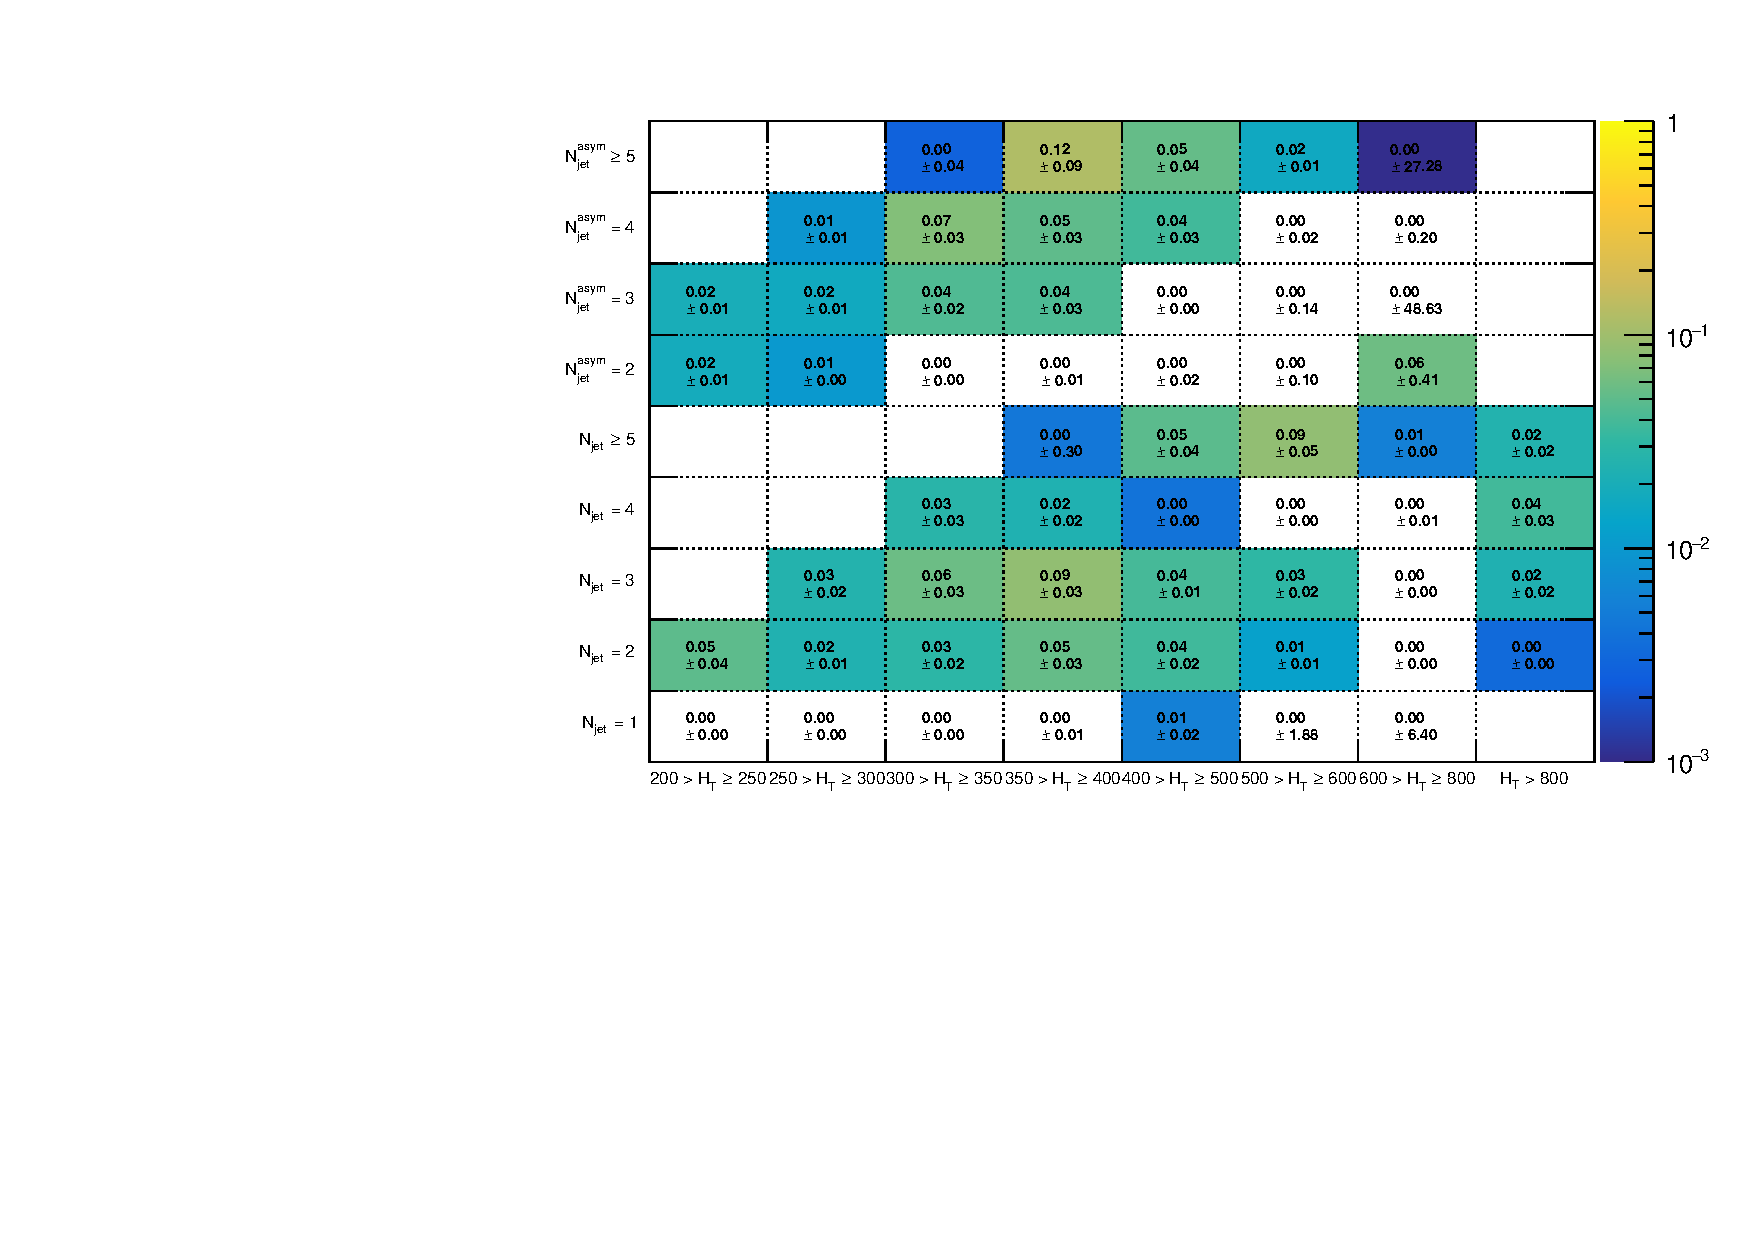
\includegraphics[width=0.49\textwidth]{figures/qcd/v0/qcd_pred} \,
    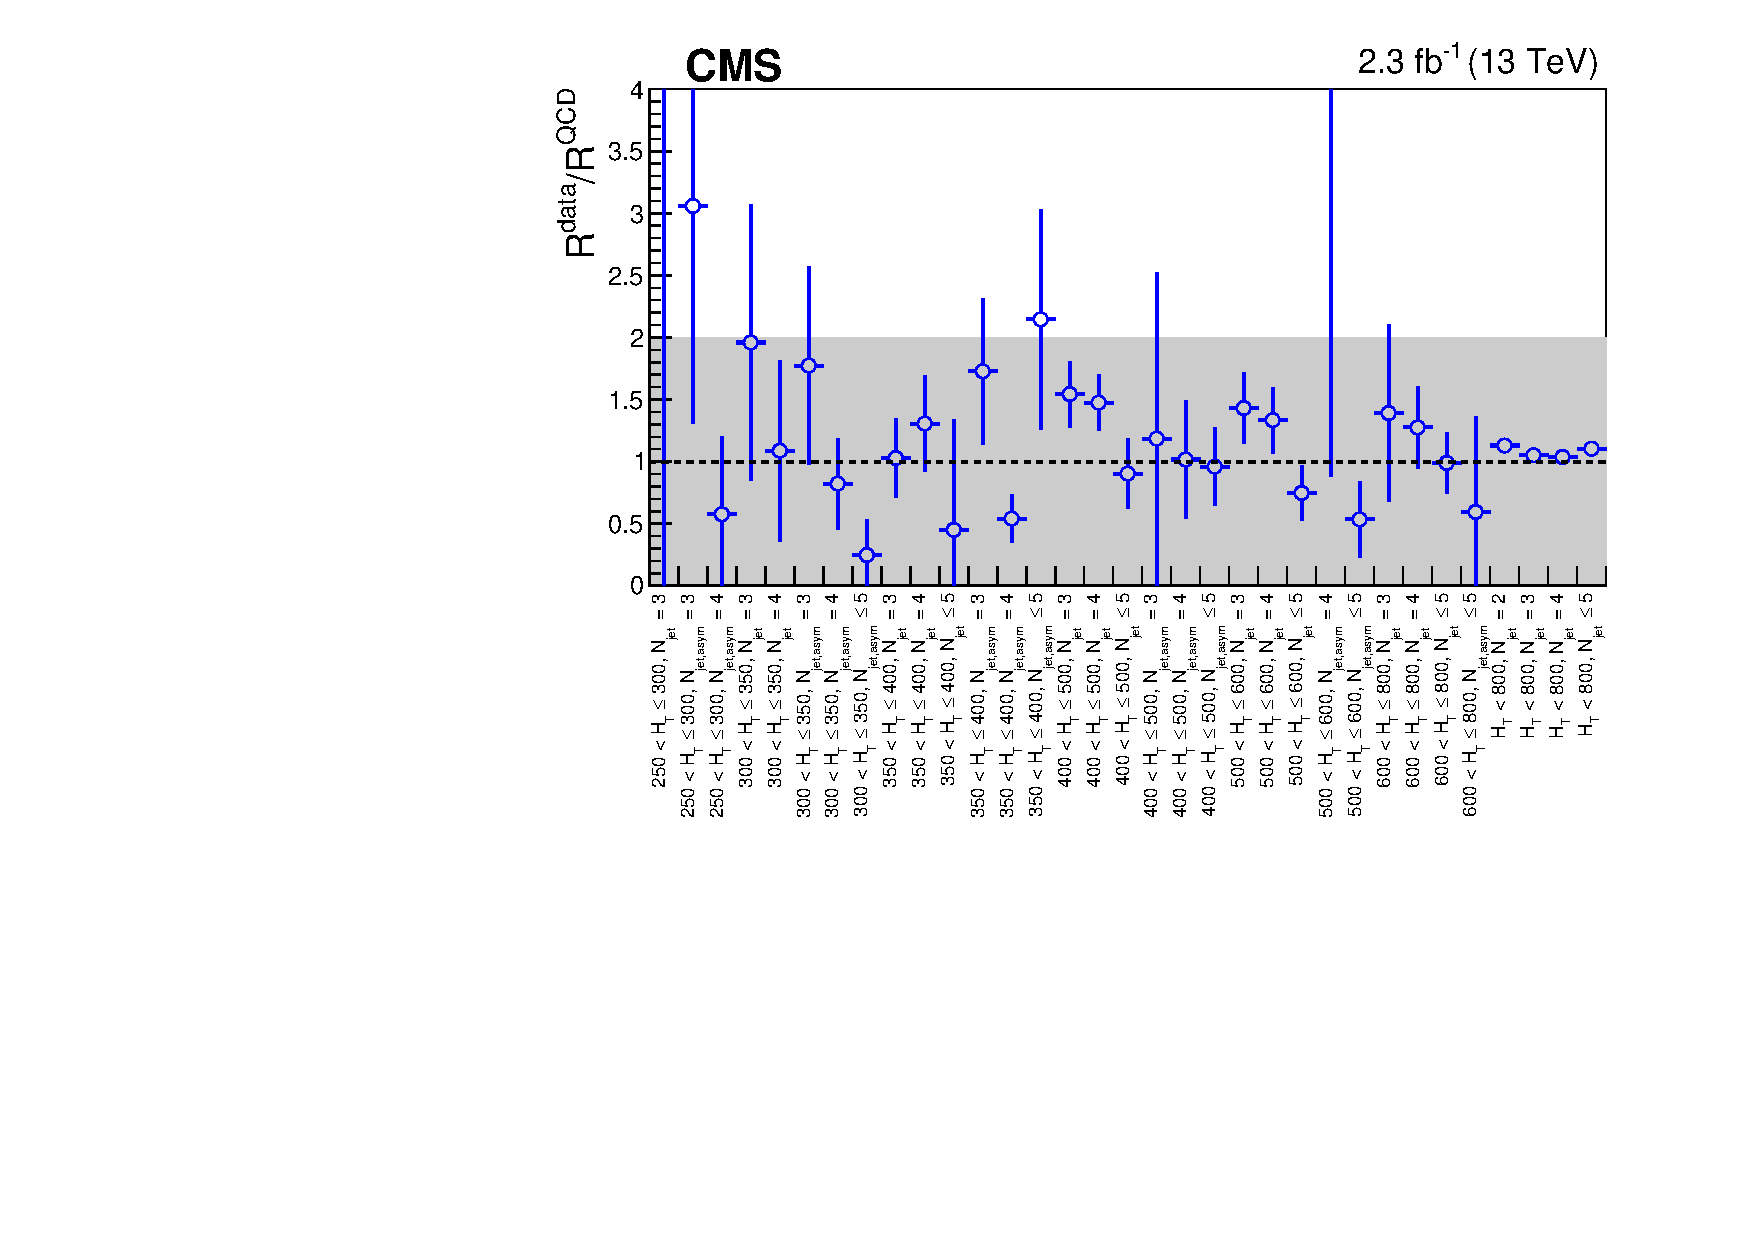
\includegraphics[width=0.7\textwidth]{figures/qcd/v3/DoubleRatioQCD_noEmpty} \\
  \end{center}
  \caption{Validation of the ratio $\mathcal{R}^\text{QCD}$ determined
    from simulation in bins of \njet and \scalht [GeV] by comparing
    with an equivalent ratio $\mathcal{R}^\text{data}$ constructed
    from data in a multijet-enriched sideband to the signal region. A
    value of unity is expected for the double ratio
    $\mathcal{R}^\text{data} / \mathcal{R}^\text{QCD}$, and the grey
    shaded band represents the assumed systematic uncertainty of 100\%
    in $\mathcal{R}^\text{QCD}$.  }
  \label{fig:qcd} 
\end{figure}

The use of simulation to determine $\mathcal{R}^\text{QCD}(\njet,
\scalht)$ is validated using a multijet-enriched data sideband defined
by $\bdphi < 0.5$.
%and an \alphat requirement identical to that used for the signal
%region, which is dependent on the value \scalht, as summarised in
%Table~\ref{}. 
Each ratio $\mathcal{R}^\text{data}(\njet, \scalht)$ is constructed
from data counts, corrected to account for contributions from
nonmultijet processes, and compared with the corresponding ratio
$\mathcal{R}^\text{QCD}(\njet, \scalht)$, determined from simulation,
through the double ratio
$\mathcal{R}^\text{data}/\mathcal{R}^\text{QCD}$, as shown in
Fig.~\ref{fig:qcd}. The double ratios are statistically compatible
with unity across the full phase space of the signal region, including
the bins at high \scalht, which exhibit the highest statistical
precision. In addition to statistical uncertainties as large as
$\sim$100\%, a systematic uncertainty of 100\% in
$\mathcal{R}^\text{QCD}$ is assumed to adequately cover the observed
level of agreement for the full signal region phase space, as well as
any limitations in the assumptions concerning $\mathcal{K}_{\njet,
  \scalht}(\nb, \HTmiss)$ for all event categories defined in terms of
\njet and \scalht.

%Finally, data control variables, such as $\bdphimod$, are inspected
%for localised populations in $(\eta,\phi)$-space to provide confidence
%that any multijet contamination due to instrumental effects is
%negligible.
